% !TEX root = ../main.tex
\begin{frame}\begin{center}
\LARGE\textbf{Example}
\end{center}\end{frame}
%-------------------------------------------------------------------------------
%-------------------------------------------------------------------------------
\begin{frame}\textbf{Seminal paper}\vspace{0.3cm}

\begin{itemize}\setlength\itemsep{1em}
\item Keane, M. P. \& Wolpin, K. I. (1994). The solution and estimation of discrete choice dynamic programming models by simulation and interpolation: Monte Carlo evidence. \textit{Review of Economics and Statistics},  76 (4), 648-672.
\end{itemize}
\end{frame}
%-------------------------------------------------------------------------------
%-------------------------------------------------------------------------------
\begin{frame}\textbf{Skill Production Function}\vspace{0.3cm}

\begin{align*}
e_{j,k,t} & =  \exp\{ \underbrace{e_{j,k,16}}_{\text{endowment}}+ \underbrace{\alpha_{j,1} g_t + \alpha_{j,2} \Ind[g_t \geq 12] + \alpha_{j,3} \Ind[g_t \geq 16]}_{\text{schooling}}\\
                & + \underbrace{\alpha_{j,4} x_{j,t} + \alpha_{j,5} x^2_{j, t} + \alpha_{j,6} \Ind[x_{j, t} > 0] + \alpha_{j,7} x_{j\neq j^\prime, t}}_{\text{work experience}}  \\
                & + \underbrace{\alpha_{j,8}\Ind[a_{t - 1} \neq j] }_{\text{depreciation}} + \underbrace{\alpha_{j,9} (t - 16)}_{\text{age}} + \hdots + \underbrace{\epsilon_{j, t}}_{\text{risk}}\}
\end{align*}

\end{frame}
%-------------------------------------------------------------------------------
%-------------------------------------------------------------------------------
\begin{frame}
  \textbf{Reward functions}\vspace{0.5cm}

  \begin{align*}
  r_t(s_t, a_t) = \begin{cases} w_{1t} =
  \exp\{\alpha_{10} + \alpha_{11}g_t + \alpha_{12}e_{1t} + \alpha_{13}e^2_{1t} + \alpha_{14}e_{2t} + alpha_{15}e^2_{2t} + \epsilon_{1t}\} & \text{if}\; a_t = 1 \\
  w_{2t} = \exp\{\alpha_{20} + \alpha_{21}g_t + \alpha_{22}e_{1t} + \alpha_{23}e^2_{1t} + \alpha_{24}e_{2t} + \alpha_{25}e^2_{2t} + \epsilon_{2t}\}& \text{if}\; a_t = 2 \\
  \beta_0 - \beta_1 \Ind[\,g_t \geq 12\,] - \beta_2\Ind[\,a_{t - 1} \neq 3\,] + \epsilon_{3t}& \text{if}\; a_t = 3 \\
  \gamma_0 + \epsilon_{4t}& \text{if}\; a_t = 4. \\
  \end{cases}
  \end{align*}
\end{frame}
%-------------------------------------------------------------------------------
%-------------------------------------------------------------------------------
\begin{frame}
  \textbf{Reward functions}\vspace{0.5cm}
\begin{align*}
    e_{1,t+1} &= e_{1t} + \Ind[\,a_t = 1\,] \\
    e_{2,t+1} &= e_{2t} + \Ind[\,a_t = 2\,] \\
    g_{t+1}   &= g_{t\phantom{2}}    +  \Ind[\,a_t = 3\,]
\end{align*}
\end{frame}
%-------------------------------------------------------------------------------
%-------------------------------------------------------------------------------
\begin{frame}
  \begin{figure}
  \caption{Choices over the life cycle}\label{Choices over the life cycle}
  \scalebox{0.35}{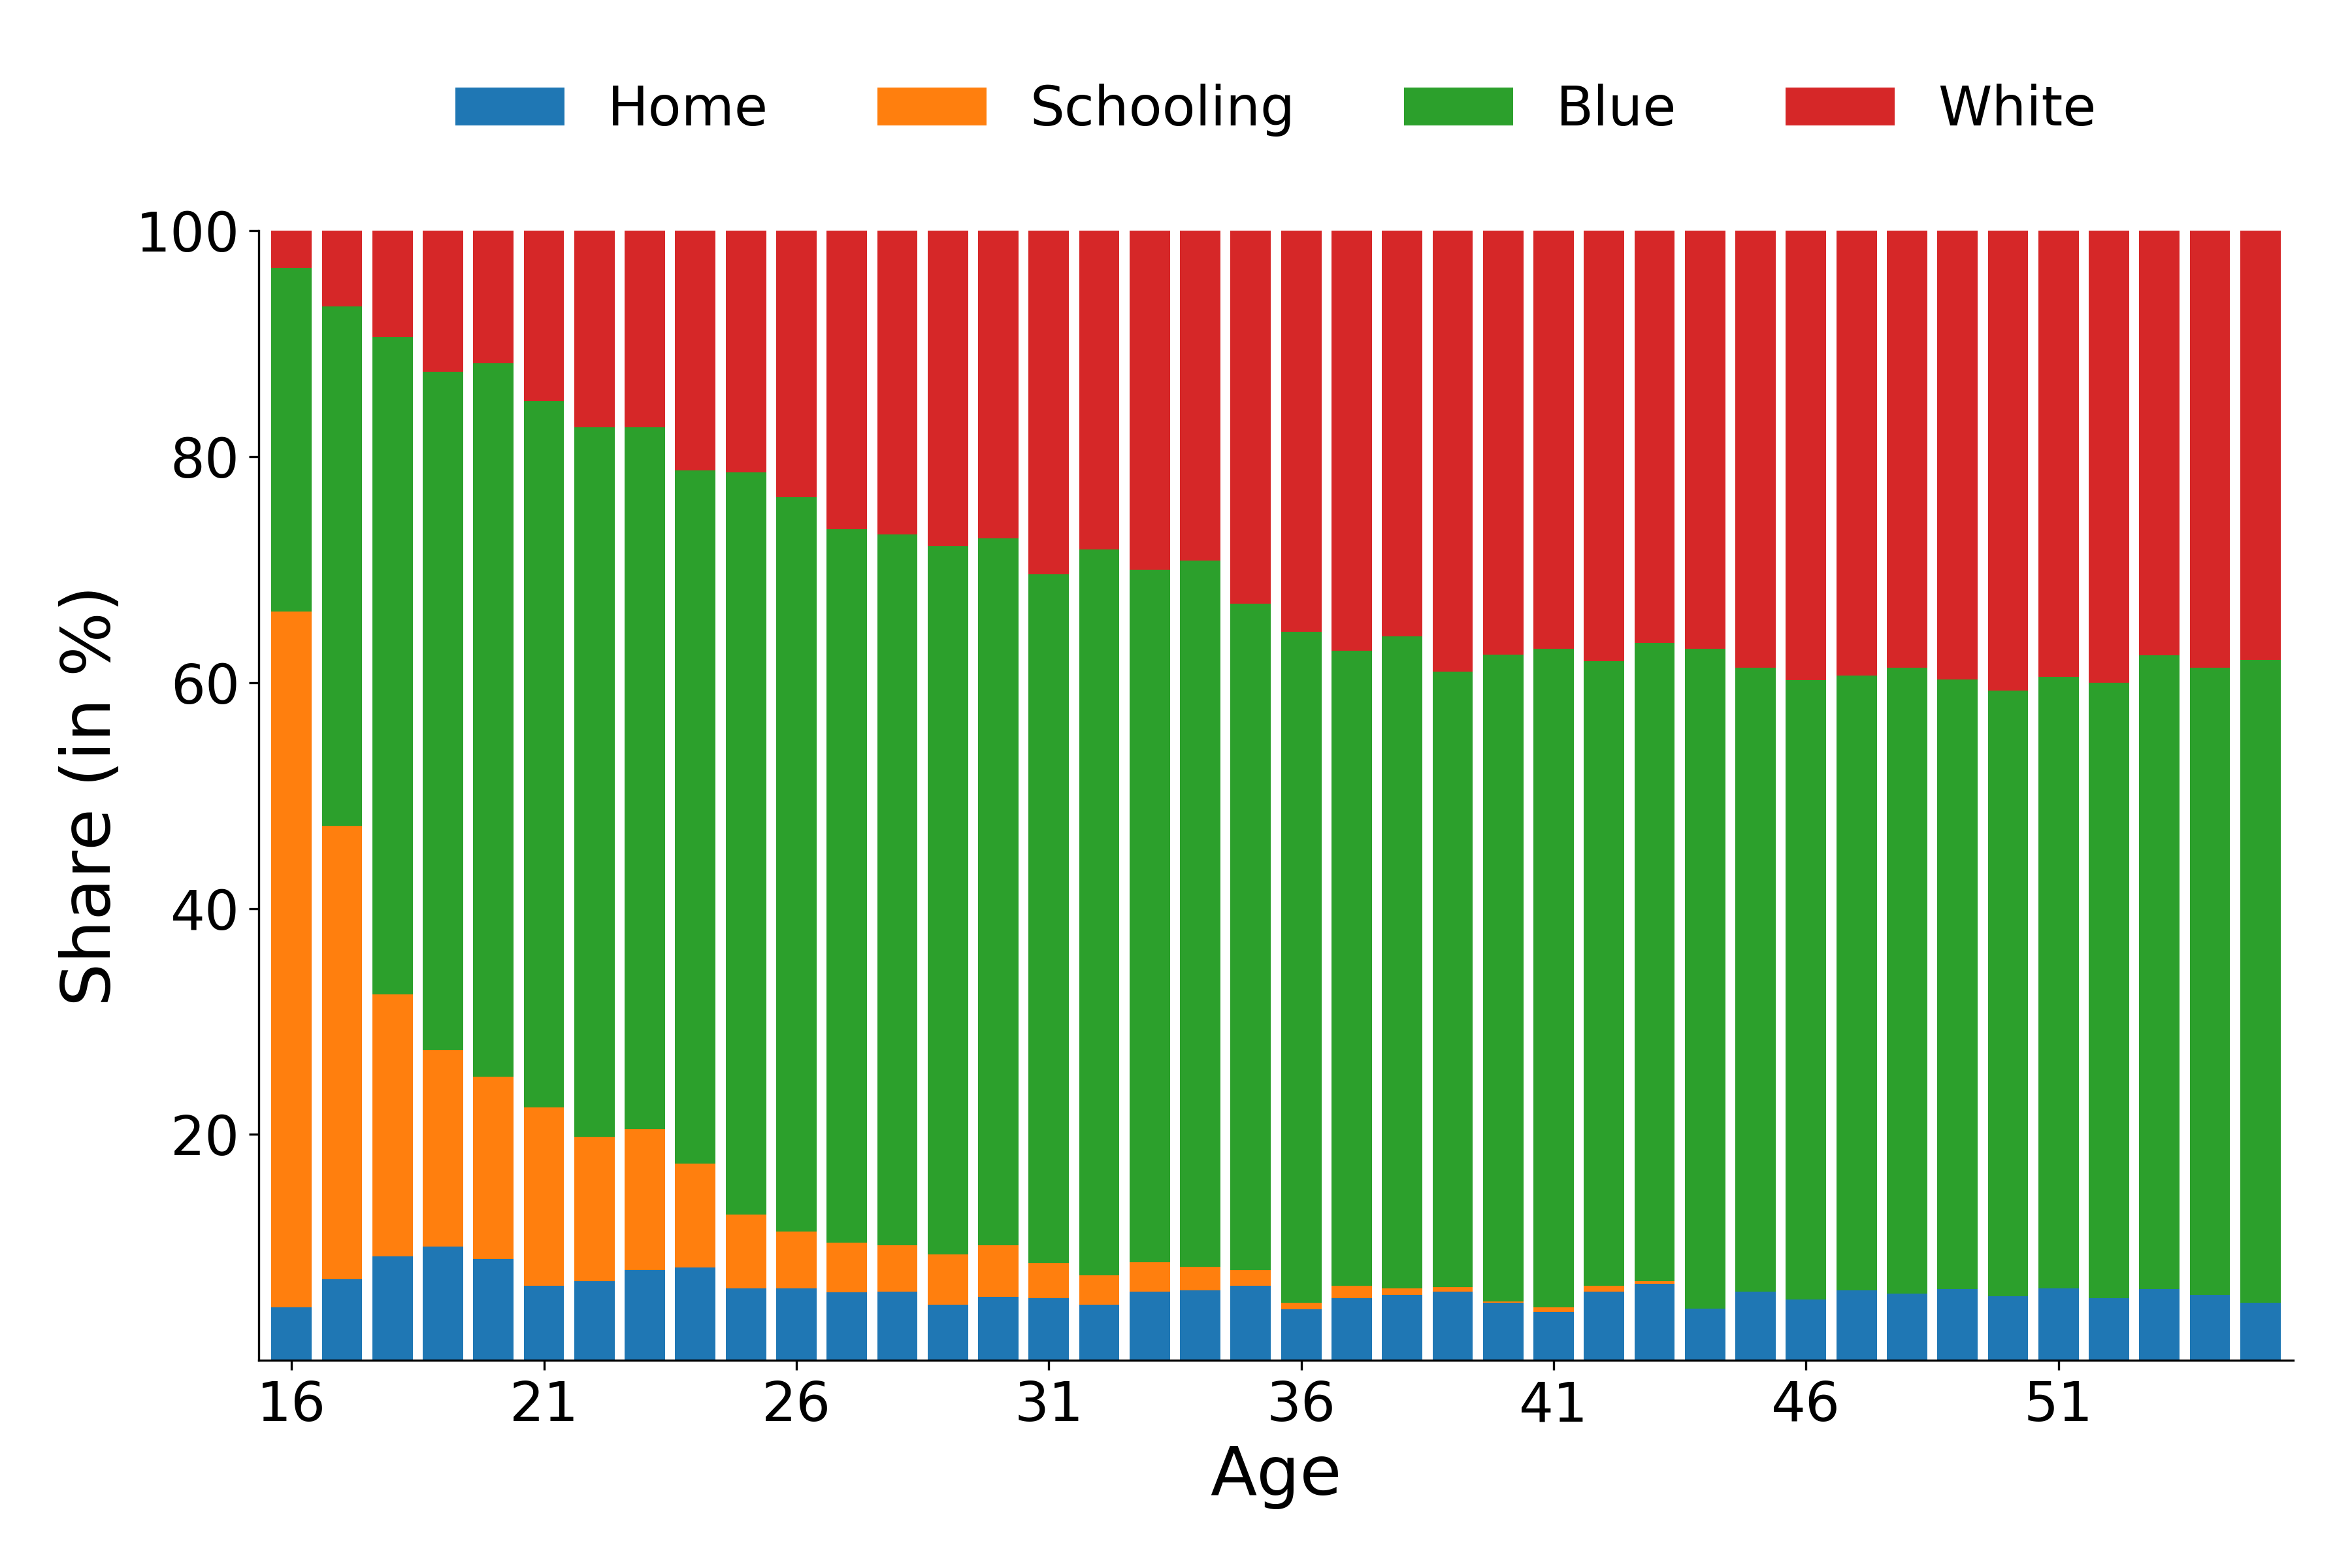
\includegraphics{fig-observed-choices-colored}}
  \end{figure}
\end{frame}
%-------------------------------------------------------------------------------
%-------------------------------------------------------------------------------
\begin{frame}
  \begin{figure}[h!]\centering
  \caption{Economic mechanism and policy forecast}\label{Economic mechanism and policy forecast}
  \subfloat[Time preference]{\scalebox{0.15}{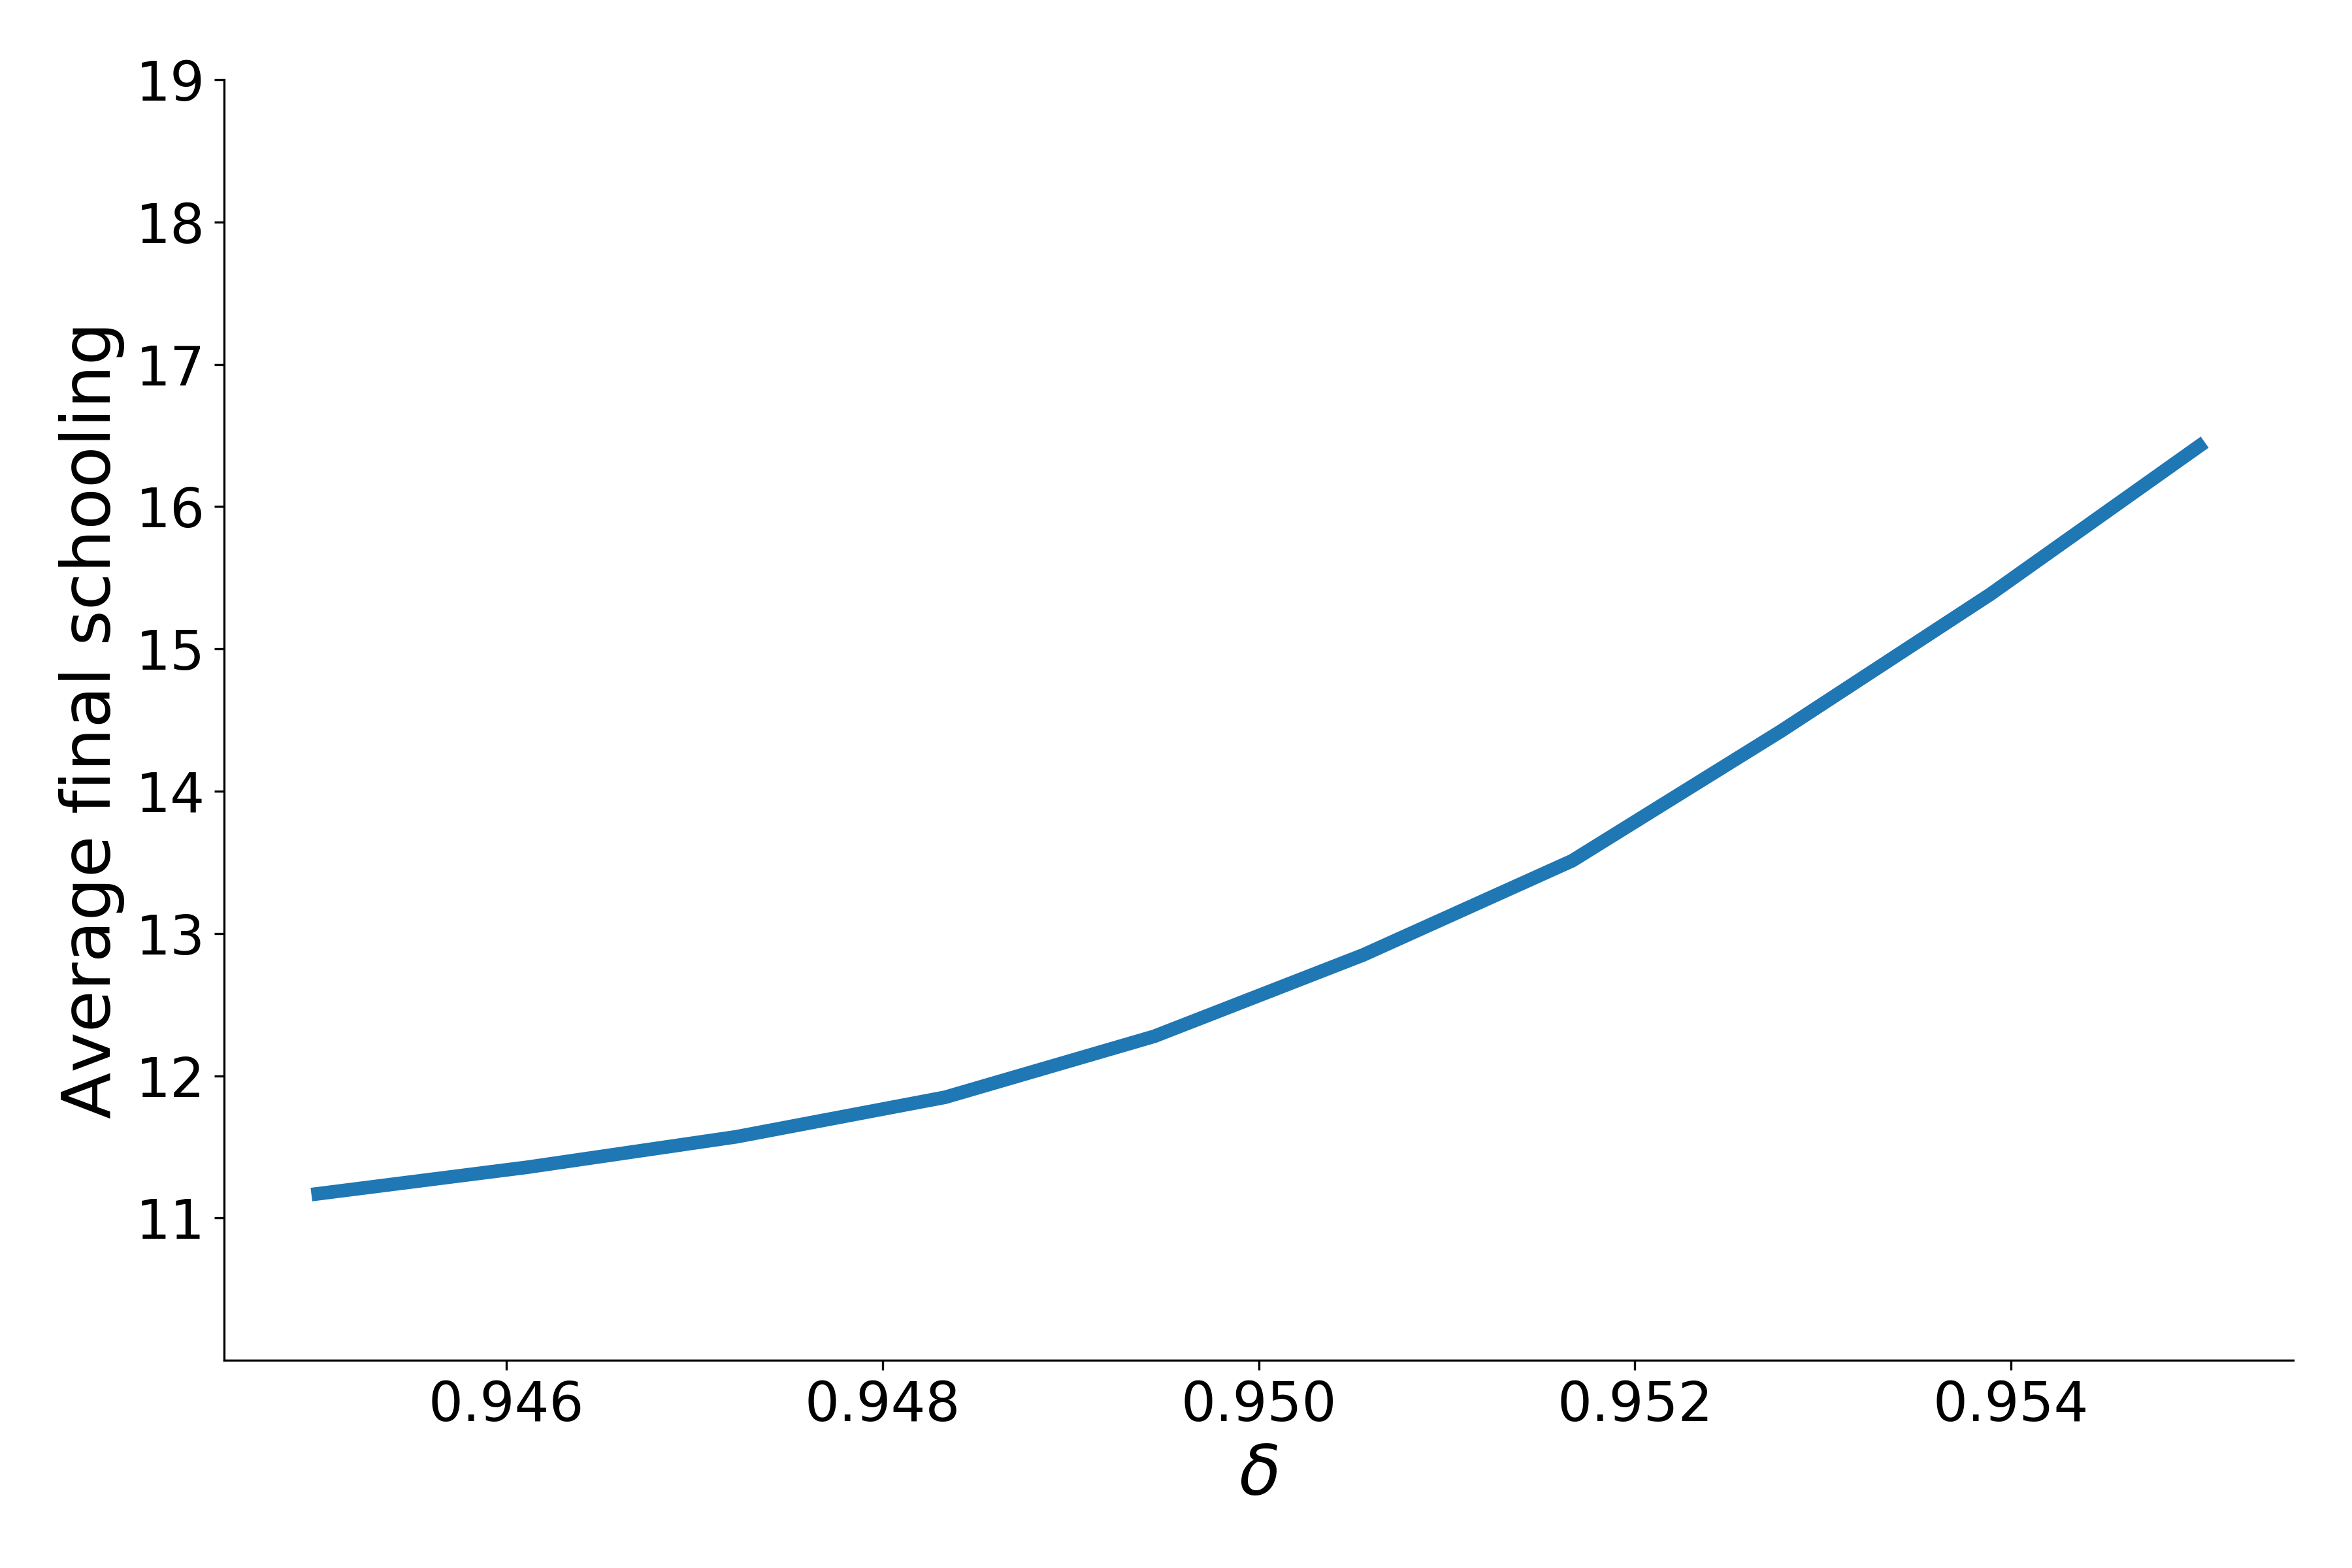
\includegraphics{fig-economic-mechanisms-colored}}}\hspace{0.3cm}
  \subfloat[Tuition subsidy]{\scalebox{0.15}{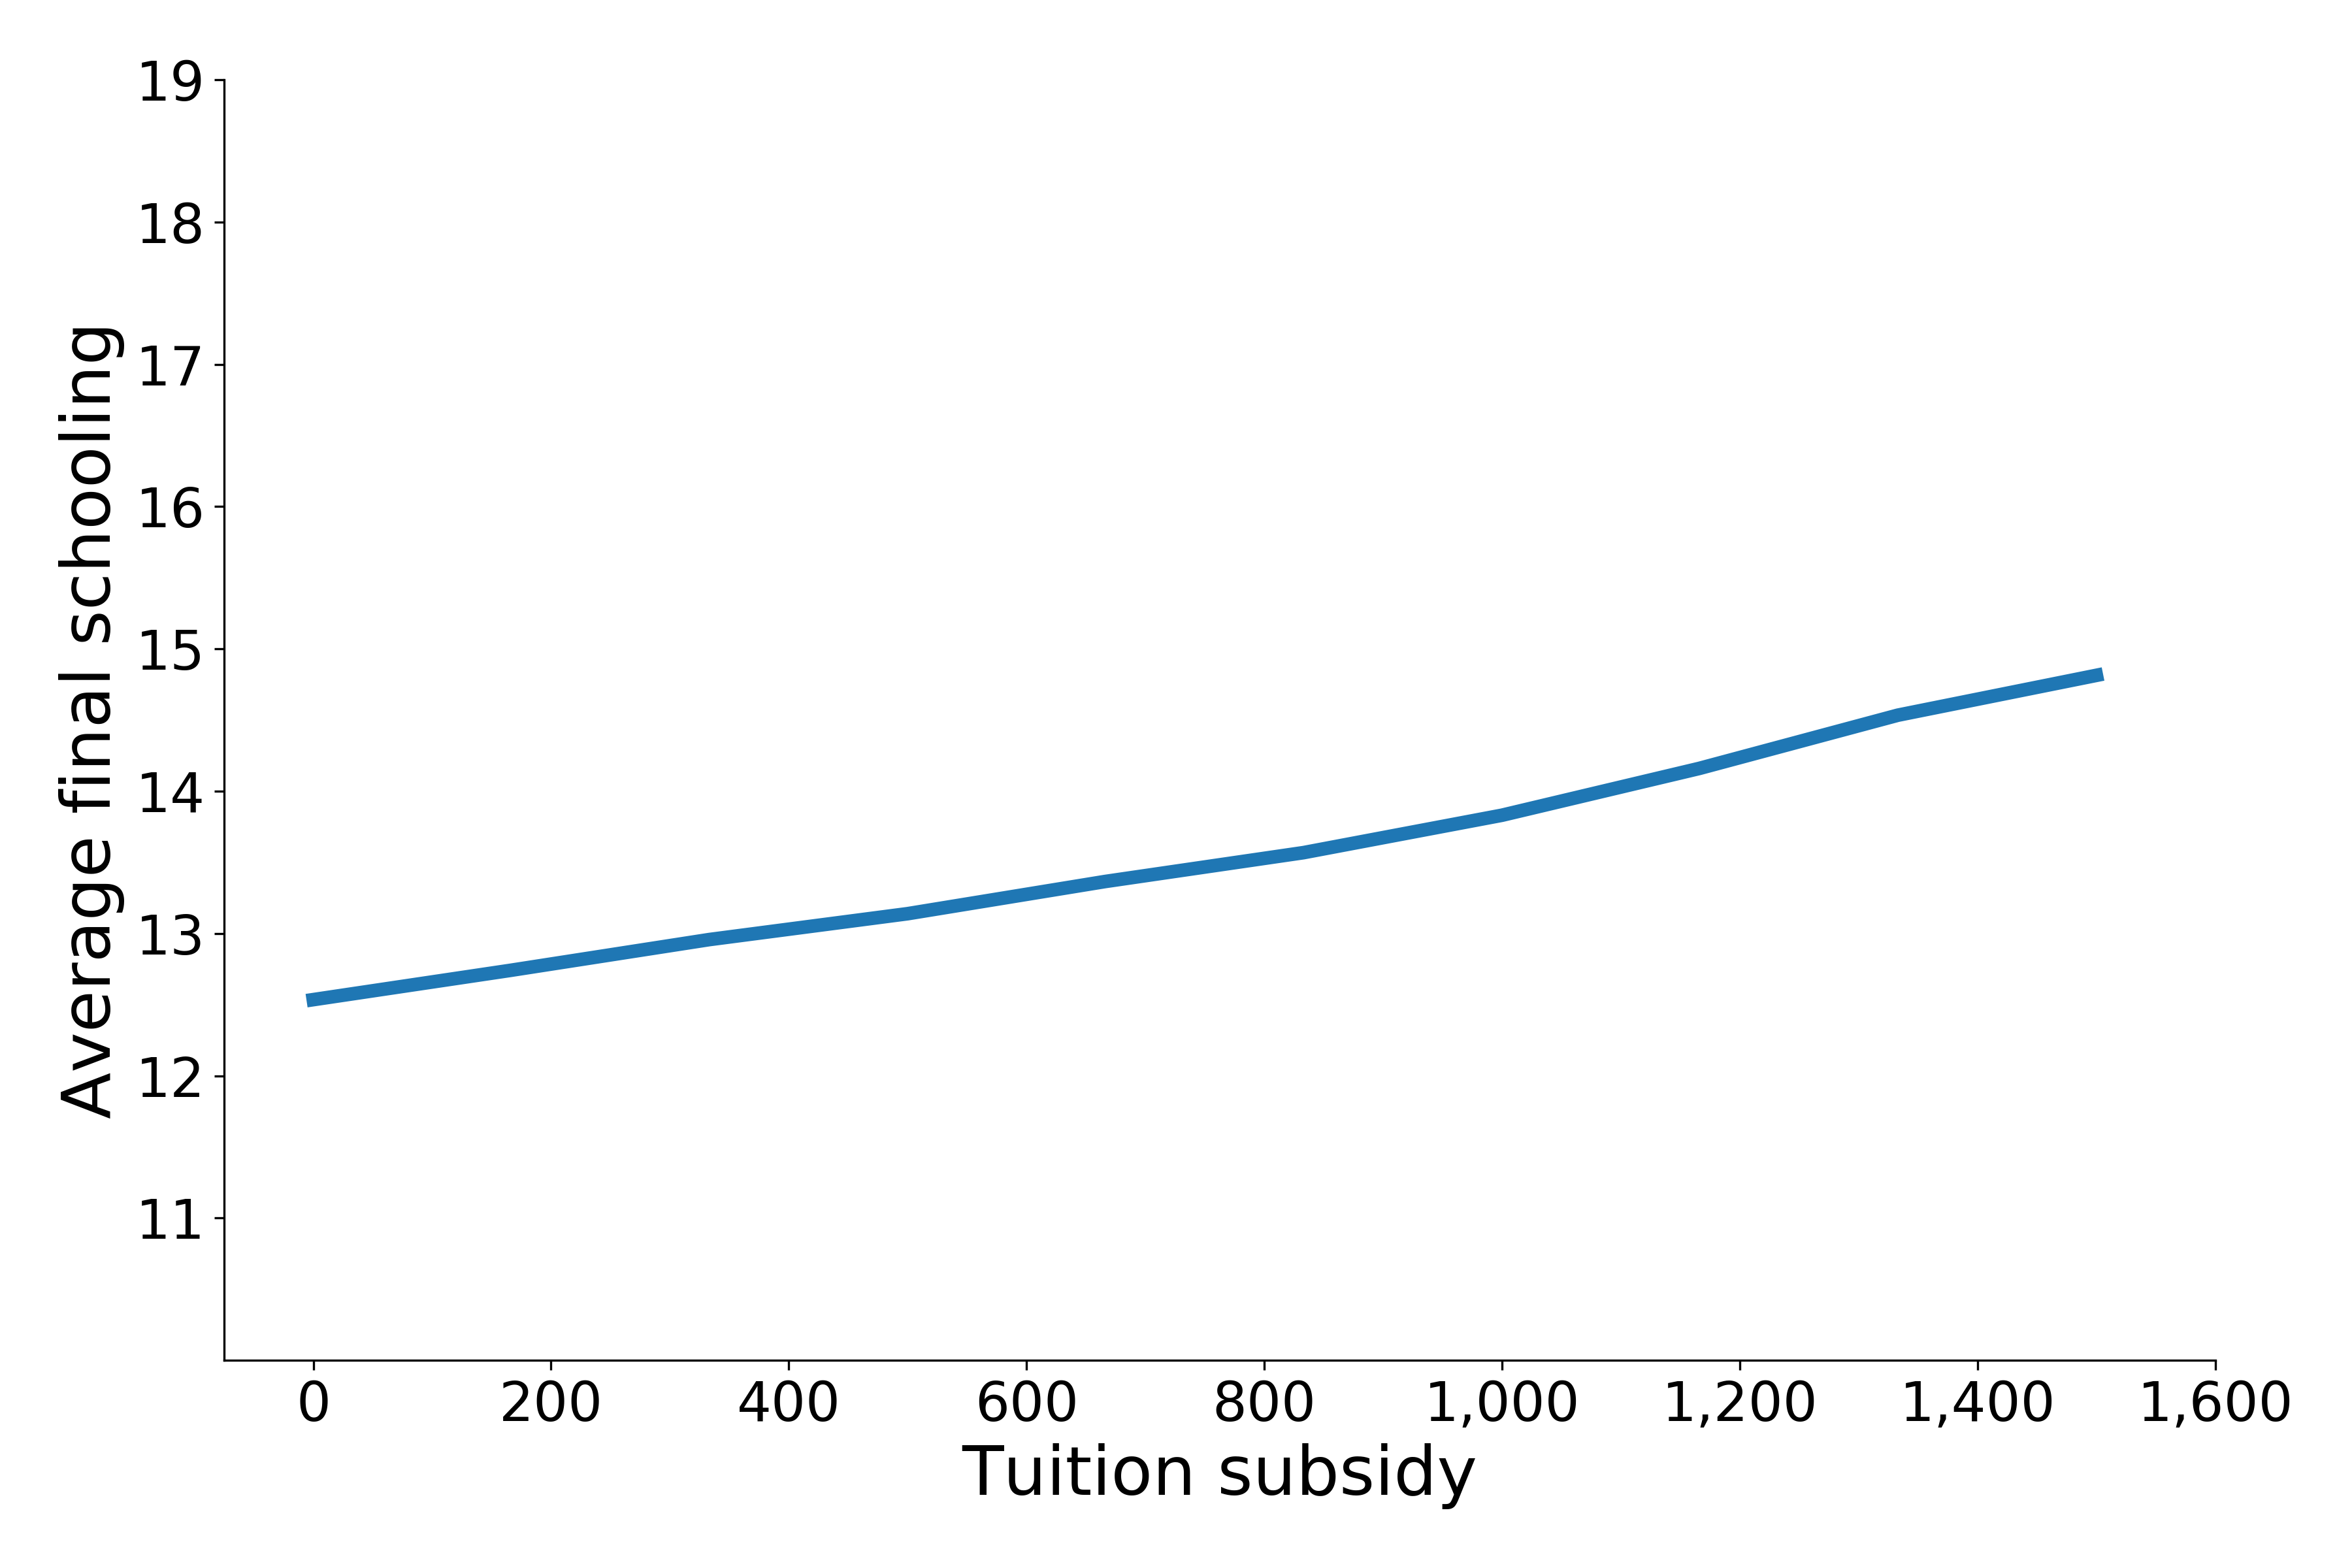
\includegraphics{fig-policy-forecast-colored}}}
  \end{figure}
\end{frame}
%-------------------------------------------------------------------------------
%-------------------------------------------------------------------------------
\begin{frame}\begin{center}
  \Large\textit{Research codes}
\end{center}\end{frame}
%-------------------------------------------------------------------------------
%-------------------------------------------------------------------------------
\begin{frame}
\textbf{respy}\\\vspace{0.3cm}
\begin{tabular}{ll}
GitHub  & \url{OpenSourceEconomics/respy}\\
Docs    & \url{respy.readthedocs.io}\\
\end{tabular}\\\vspace{1cm}

\textbf{estimagic}\\\vspace{0.3cm}
\begin{tabular}{ll}
GitHub	& \url{OpenSourceEconomics/estimagic}\\
Docs    & \url{estimagic.readthedocs.io}\\
\end{tabular}

\end{frame}
%-------------------------------------------------------------------------------
%-------------------------------------------------------------------------------
\begin{frame}
  \begin{figure}\tiny
    \caption{Typical workflow}
   \lstset{language=python, morekeywords={as}, ndkeywords={=}, ndkeywordstyle=\color{blue}, keywordstyle=\color{red}, commentstyle=\color{darkgrey}, emph={get_example_model, get_crit_func, get_simulate_func}, emphstyle=\color{violet}}
         \lstinputlisting{../material/workflow.py}
   \end{figure}
\end{frame}
%-------------------------------------------------------------------------------
%-------------------------------------------------------------------------------
\begin{frame}

  \begin{figure}[h!]\centering
  \caption{Model specification}\label{Model specification}
  \subfloat[Parameterization]{\scalebox{0.15}{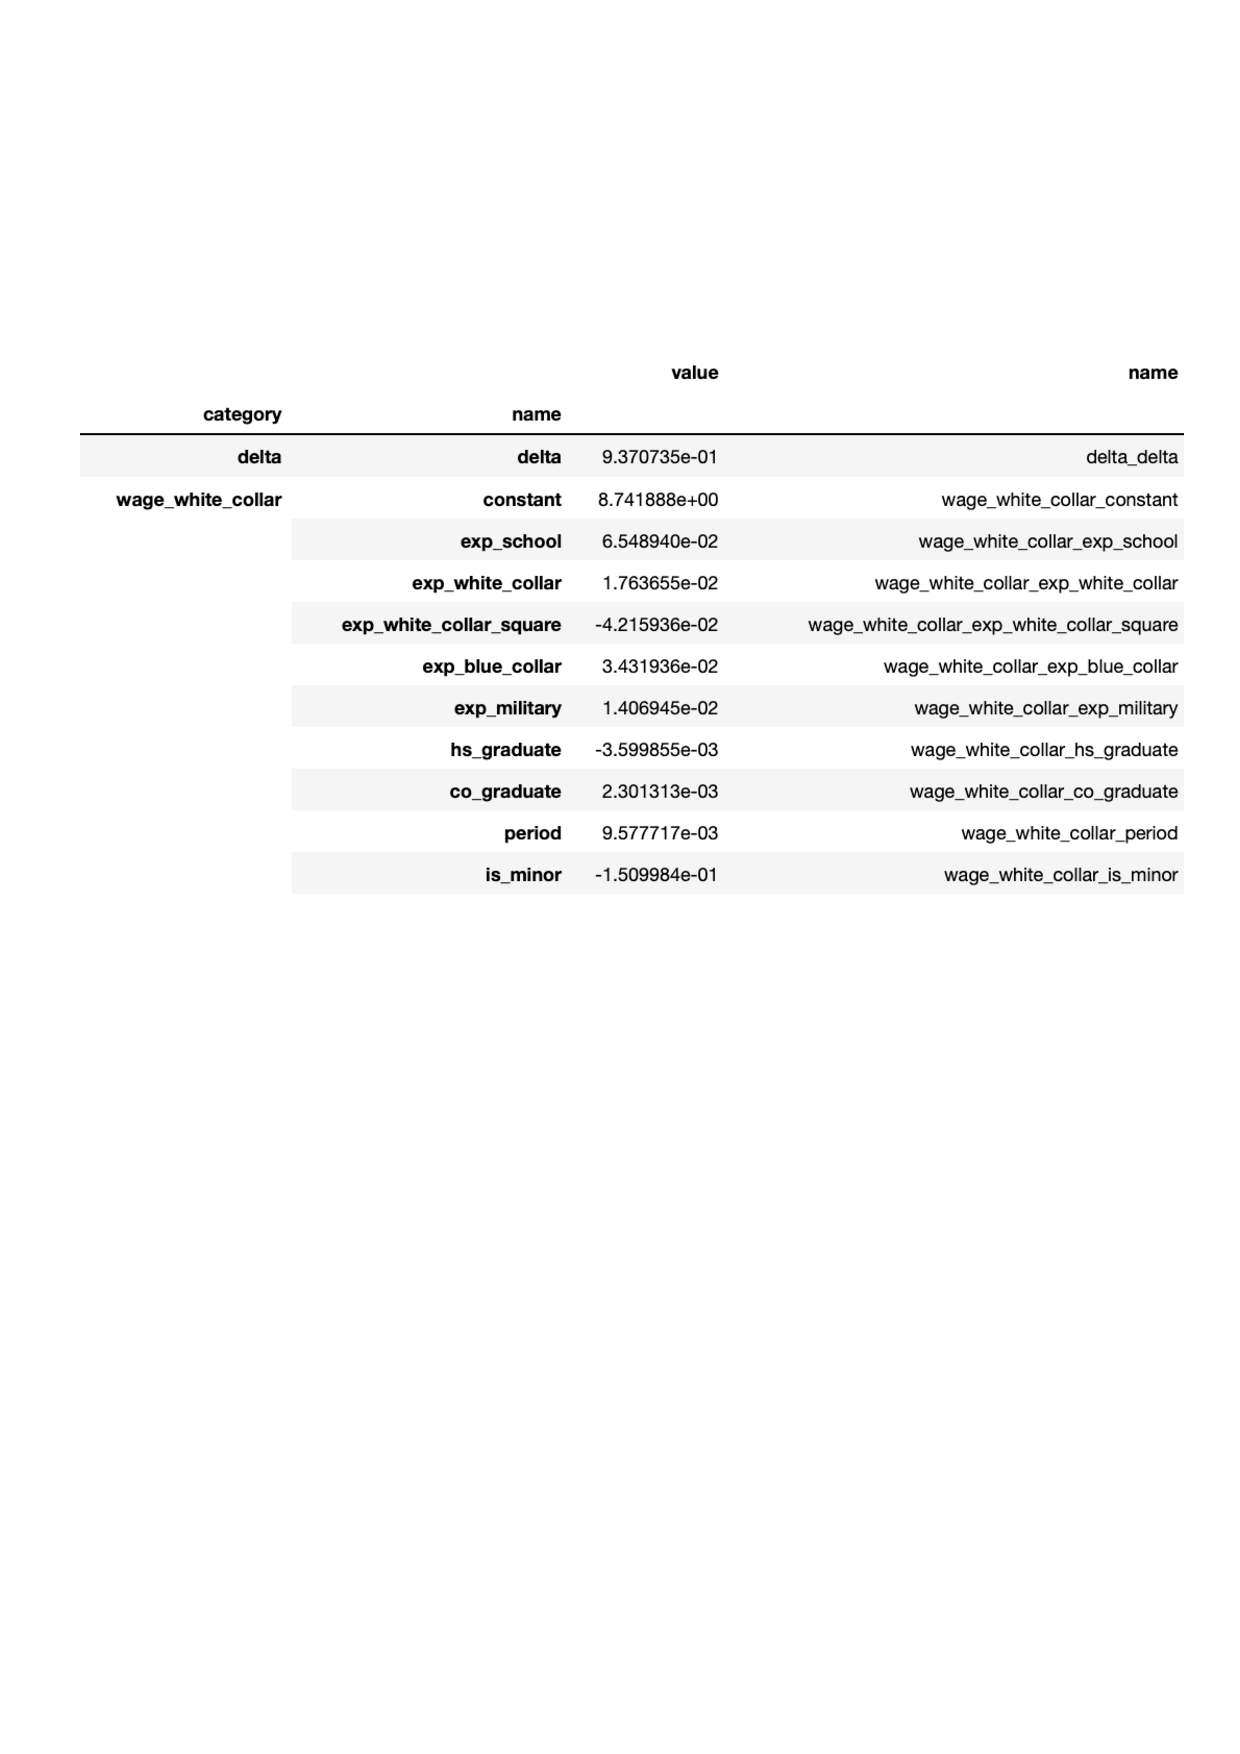
\includegraphics{crop-params}}}\hspace{0.3cm}
  \subfloat[Options]{\scalebox{0.15}{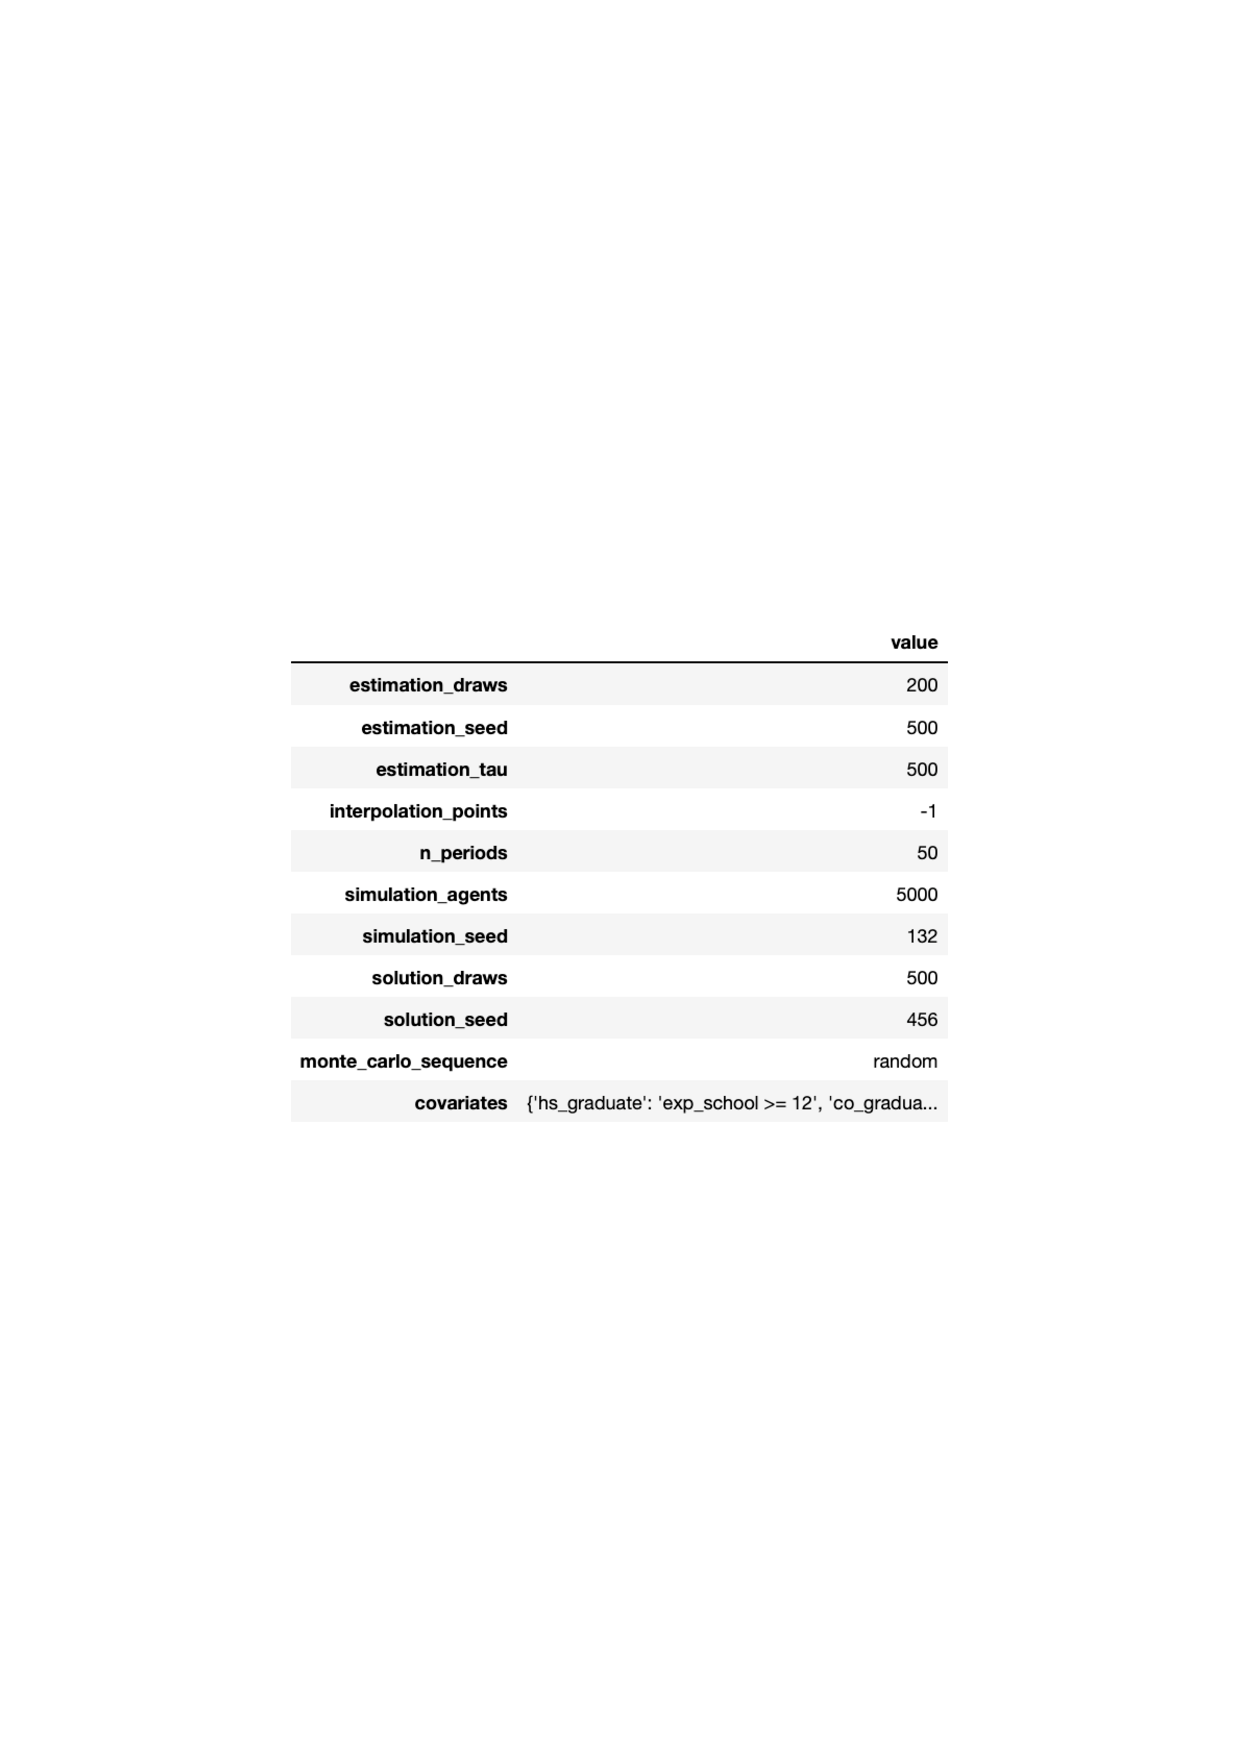
\includegraphics{crop-options}}}
  \end{figure}

\end{frame}
%-------------------------------------------------------------------------------
%-------------------------------------------------------------------------------
\begin{frame}

  \begin{figure}[h!]\centering
  \caption{Dashboard}\label{Dashboard}
  \scalebox{0.50}{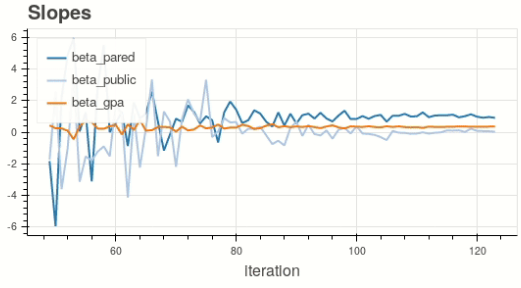
\includegraphics{crop-dashboard}}
  \end{figure}

\end{frame}
%-------------------------------------------------------------------------------
%-------------------------------------------------------------------------------
